\section{\dis Network Requirements}
\label{sec:requirements}





We start by evaluating network latency and bandwidth requirements for disaggregation.
We describe our evaluation methodology (\S\ref{ssec:rmethod}), present our results (\S\ref{ssec:rr}) and then discuss their implications (\S\ref{ssec:rtt}). 

\subsection{Methodology}
\label{ssec:rmethod}
In a disaggregated datacenter, traffic between resources that was contained within a server is now carried on the “external” network. As with other types of interconnects, the key requirement will be low latency and high throughput to enable this disaggregation. We review the forms of communication between resources within a server in Table~\ref{tab:tech} to examine the feasibility of such a network. 
We ignore for now the possible effects of network congestion which we will evaluate in \S\ref{sec:existing}.

As mentioned in \S\ref{sec:summary}, CPU-to-CPU cache coherence traffic does not cross the external traffic.
For I/O traffic to network interfaces and disks, the required latency and bandwidth is such that we can expect to consolidate them within the unified network with low performance impact. 
Thus, the dominant impact to application performance will come from disaggregating memory and hence we focus on evaluating the network bandwidth and latency required to support remote memory.

As mentioned earlier, we assume that remote memory is managed at the page granularity, in conjunction with virtual memory page replacement algorithms implemented by the hypervisor or operating system. This approach guarantees that frequently-accessed remote pages will be cached locally, and also transparently supports unmodified applications.
For each paging operation there are two main sources 
of performance penalty: i) the software overhead for trap and page eviction and ii) the time to transfer pages over the network. 
Given our focus on network requirements, we only consider the latter in this paper (modulo a brief discussion on current 
software overheads later in this section).

%
\begin{table*}
  \centering
  \small
  \begin{tabular}{c|c|c|c}
		\textbf{Application Domain} & \textbf{Application} & \textbf{System} & \textbf{Dataset} \\\hline \hline
%		\textbf{domain} & \textbf{} & \textbf{}\\
    Off-disk Batch & WordCount & Hadoop & Wikipedia edit history~\cite{wikipedia}\\\hline
    Off-disk Batch & TeraSort & Hadoop & Terasort benchmark generator\\\hline
%    In-memory Batch & WordCount & Spark & Wikipedia edit history~\cite{wikipedia}\\\hline
    Graph Processing & Collaborative Filtering & GraphLab & NetFlix movie rating data~\cite{netflix}\\\hline
    Point Queries & Key-value store & Memcached & YCSB benchmark B\\\hline
    % Point Queries & Search & ElasticSearch & PS\\\hline
    % Stream Processing & Wordcount & Storm & S\\\hline
    \hline
  \end{tabular}
  \vspace{0.1in}
  \caption{\small{Applications, workloads, systems and datasets used in our study.}}
  \label{tab:workloads}
\end{table*}

%

\paragraphb{Applications and testbed}
We conduct a series of experiments to examine how network latency and bandwidth affect application performance with remote memory accesses (which we emulate as described below). 
We use workloads from diverse applications running on real-world and benchmark datasets, as shown in Table~\ref{tab:workloads}. %These workloads constitute a wide variety of application domains including off-disk batch processing (Hadoop), in-memory batch processing (Spark), graph processing (GraphLab) and point queries (memcached).
 Each application operates on $125$GB of data equally distributed across an Amazon EC2 cluster comprising of $5$ m3.2xlarge servers. Each of these servers has $8$ vCPUs, $30$GB main memory, $2 \times 80$GB SSD drives and a $1$Gbps access link bandwidth.
 We enabled EC2's Virtual Private Network (VPC~\cite{vpc}) capability in our cluster, ensuring no interference with other Amazon EC2 machines. 



\paragraphb{Emulating remote memory} 
When running the above workloads, we emulate remote memory accesses by implementing a special swap device that is backed by physical memory rather than a disk. This effectively partitions main memory into a ``local'' and ``remote'' portion 
with existing page replacement algorithms controlling when and how pages are transferred between the two; we tune the amount of `local' memory by configuring the size of the swap device (our `remote' memory).
We intercept all page faults and inject artificial delays to emulate network round-trip latency and bandwidth for each paging operation. 

We measure relative performance on the basis of throughput or completion time as compared to the zero-delay case. Thus our results do not account for the delay introduced by  software overheads for page operations 
and should be interpreted as relative performance degradation over different network configurations.%, not the absolute performance of disaggregation.
Note too that the delay we inject is purely an artificial parameter and hence doesn't (for example) realistically model queueing delays that may result from network congestion caused by the extra traffic due to disaggregation; we consider network-wide traffic and effects such as congestion in the sections to follow.


%using an in-house implementation of a light-weight special instrumentation tool (SIT) that runs atop existing servers. SIT

%and records the time and memory addresses accessed by the application. Given our assumption of remote memory access granularity being a page size, the accessed memory addresses are translated into page-level requests (number of pages requested). 
%SIT intercepting all ``remote memory'' flows allows us to inject artificial delays to emulate resource disaggregation. 

\cut{
We inject delays due to:

\begin{itemize}[leftmargin=*]
	\itemsep0em
	\item Network end-to-end latency, which is fixed for each request. We vary end-to-end latency only across experiments.
	\item Transmission time for requests, which depends both on the access link bandwidth as well as number of pages accessed in the request. For a given request, we insert (\#pages $\times$ page-size)/(bandwidth) amount of latency.
\end{itemize}

\noindent
}
%Using the above methodology, each blade essentially experiences a disaggregated network with a constant end-to-end latency, and a fixed transmission time for a given request. 



 %\rc{The cluster is set up with Virtual Private Network (VPC) enabled, ensuring no interference with machines outside our cluster. $\gets$ apparently, not for all experiments}

\cut{
\begin{figure}
	\centering
	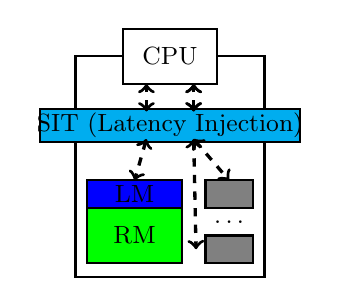
\begin{tikzpicture}[xscale=0.6, yscale=0.35]

	\draw[thick, fill=white] (-3, 5) rectangle (1, 13); 
	\draw[thick, fill=white] (-2, 14) rectangle (0, 12); 
	\draw (-1, 13) node {\small{CPU}};
	% \draw (-1, 10.5) node {\small{Handler}};
	
	\draw[thick, fill=cyan] (-3.75, 9.9) rectangle (1.75, 11.1); 
	\draw (-1, 10.5) node {\small{SIT (Latency Injection)}};
			
	\draw[thick, fill=blue] (-2.75, 7.5) rectangle (-0.75, 8.5);
	\draw[thick, fill=green] (-2.75, 5.5) rectangle (-0.75, 7.5);
	\draw (-1.75, 8) node {\small{LM}};
%	\draw (-2.75, 7.5) -- (-0.75, 7.5);
	\draw (-1.75, 6.5) node {\small{RM}};
%	\draw (-2.75, 6.5) -- (-0.75, 6.5);
%	\draw (-1.75, 6) node {\small{K$\to$O}};

%	\draw[thick] (-0.25, 5.5) rectangle (0.75, 8.5);
	\draw[thick, fill=gray] (-0.25, 8.5) rectangle (0.75, 7.5);
	\draw[thick, fill=gray] (-0.25, 5.5) rectangle (0.75, 6.5);
	\draw (0.25, 7) node {\small{$\dots$}};

	\draw[very thick, black, dashed, <->] (-1.5, 10) -- (-1.75, 8.5);
	\draw[very thick, black, dashed, <->] (-0.5, 10) -- (0.25, 8.5);
	\draw[very thick, black, dashed, <->] (-0.5, 10) -- (-0.45, 6);

	\draw[very thick, black, dashed, <->] (-1.5, 11) -- (-1.5, 12);
	\draw[very thick, black, dashed, <->] (-0.5, 11) -- (-0.5, 12);
	\draw[very thick, black, dashed, <->] (-0.5, 11) -- (-0.5, 12);

	\end{tikzpicture}
	    \caption{\small{We run real-world applications on a $5$-node Amazon EC2 cluster. To emulate end-to-end network latency, we inject artificial latencies for all ``remote memory'' and ``remote disk'' accesses and measure the impact of this latency to the application-level performance. \rc{SIT representation imprecise}}}
	\label{fig:system1}
\end{figure}}
%

\subsection{Results}
\label{ssec:rr}
\cut{
We now evaluate the network requirements in \dis, in terms of latency and bandwidth, to main application-level performance comparable to current datacenters. As briefly discussed earlier, the size of local cache on CPU blades is likely to have the biggest impact on network requirements. 
}

\paragraphb{Impact of local memory size}
We start our evaluation by studying the impact of local memory on application-level performance.
We fix the latency and bandwidth that we inject to be $5\mu$s and $40$Gbps (we pick these values for reasons described below) and measure degradation in application-level performance as the fraction of local memory is varied from $100\%$ (which corresponds to no CPU-memory disaggregation) down to $10\%$.
% of the available main memory{\footnote{The $100\%$ local CPU cache size corresponds to no CPU-memory disaggregation, as in server-centric architectures.} \rc{Shall we say that we use this as our baseline, rather than application-level performance without SIT, to incorporate SIT overhead. (a+x)/(b+x) problem.}}}. 
Figure~\ref{fig:impb} shows that the application-level performance in \dis is within reasonable bounds ($5$--$10\%$) of that in a server-centric architecture as long as the local memory cache is no smaller than $25\%$ of main memory. For larger local cache sizes, performance only improves slowly and for any smaller cache size, the performance degrades significantly. 
We conclude that \emph{a local memory cache that is sized at $25\%$ of current main memory is sufficient} to maintain reasonable application-level performance in \dis. In what follows, unless stated otherwise, we set the local memory size to this value.

%
\begin{figure}
  \centering
    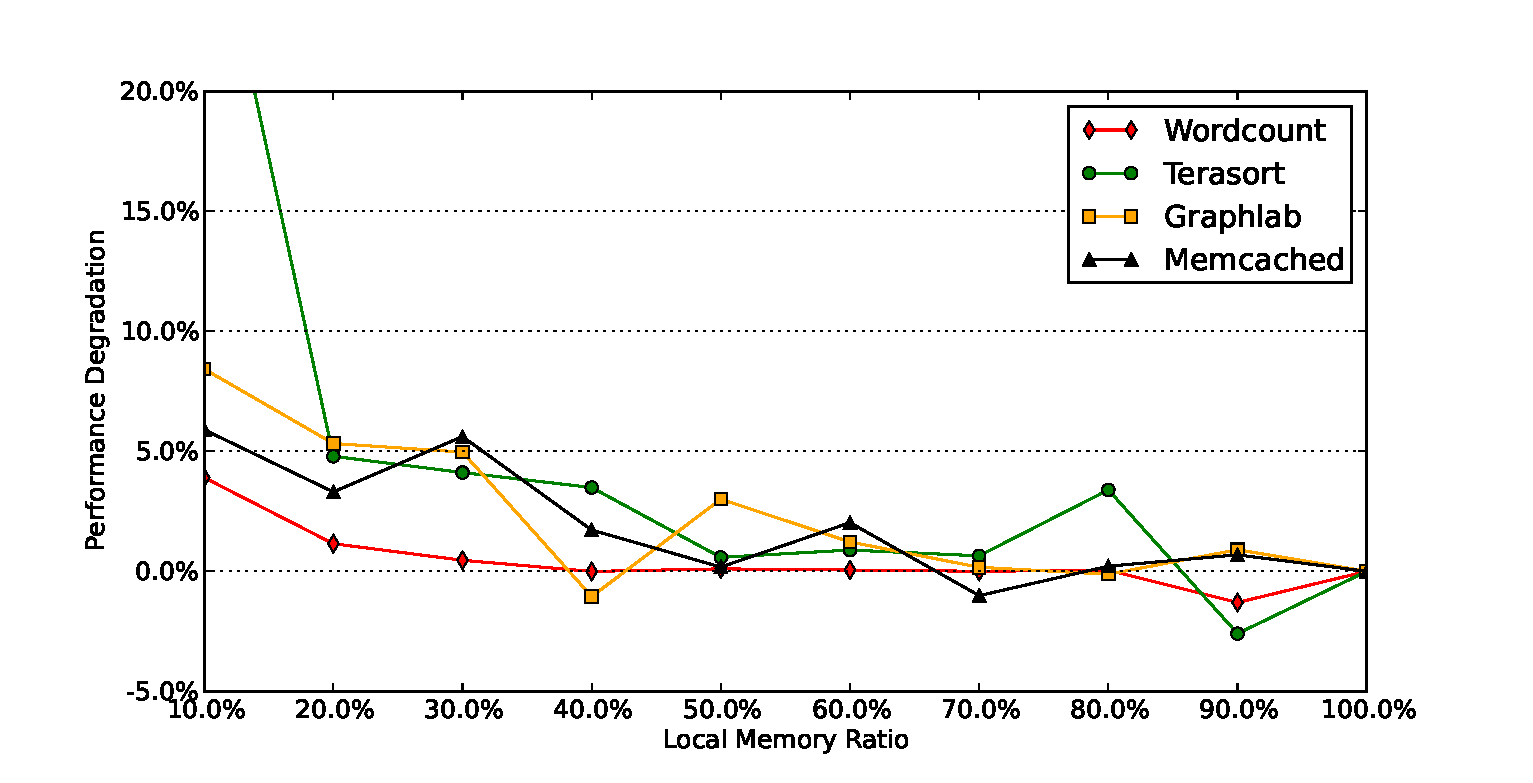
\includegraphics[width = 3.5in]{img/vary_remote_mem.eps} 
  \caption{\small{Varying the portion of local memory from 10\% to 100\%, the figure shows the application performance degradation with 5$\mu$s end-to-end network latency and 40Gbps bandwidth. With 25\% of the total memory local, the performance degredation is within 5\% to 10\%. }}
  \label{fig:impb}
\end{figure}
%
%
\begin{figure*}

  \centering
  \subfigure{
    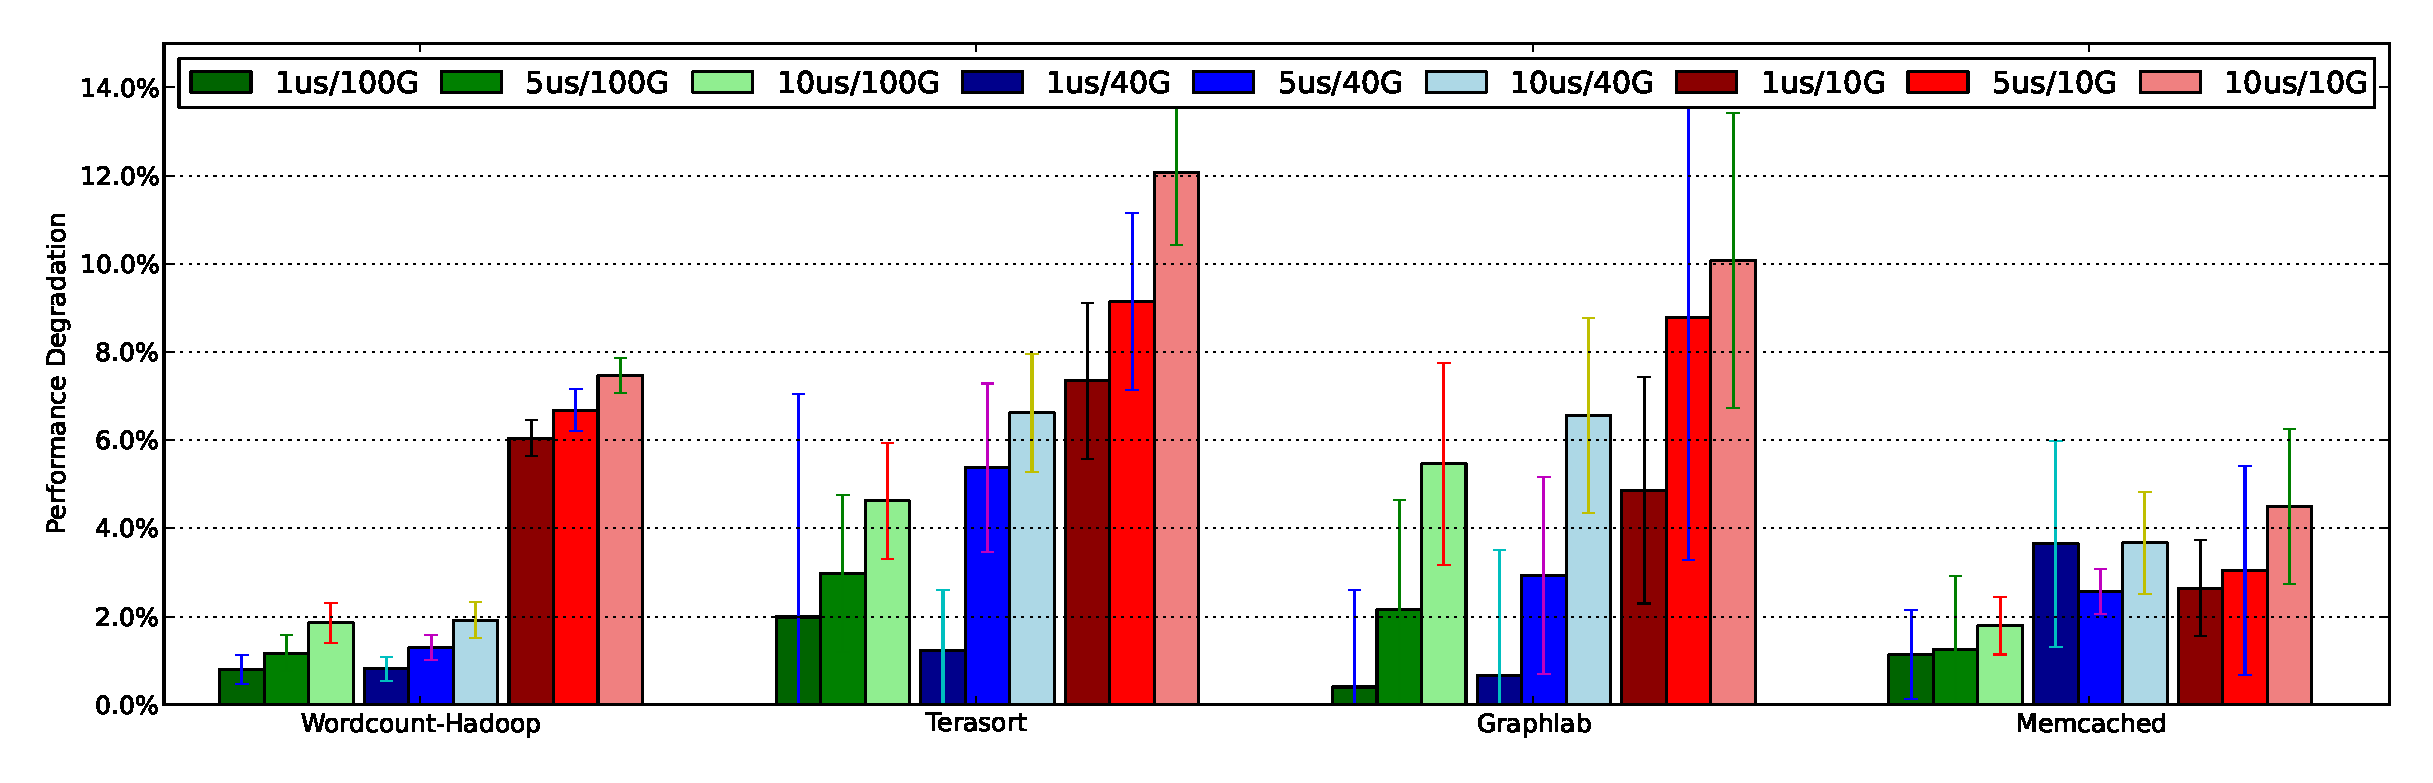
\includegraphics[height = 1.5in]{img/vary_latency_bw.eps}  
  }
%\hspace{0.05in}
%  \subfigure{
%    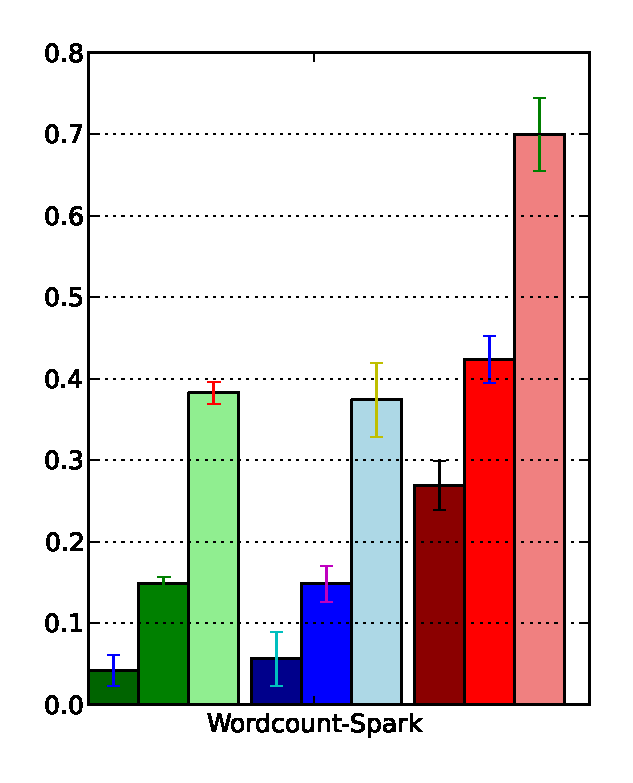
\includegraphics[height = 1.5in]{img/vary_latency_bw_spark.eps}
%  }
  \caption{\small{For a \dis with $5\mu$s end-to-end network latency and $40$Gbps access link bandwidth, the application-level performance remains within $5\%$ of current server-centric architectures for all but in-memory batch processing systems.}}
  \label{fig:latb}
\end{figure*}
%
\paragraphb{End-to-end latency and bandwidth requirements} 
%$5\mu$s end-to-end latency and $40$Gbps access link bandwidth is sufficient}
Figure~\ref{fig:latb} shows the performance degradation that results with nine different latency/bandwidth combinations, given 25\% of memory capacity as local.% of the measured memory footprint for each workload. 
%We now evaluate the application-level performance for various \dis configurations in terms of end-to-end network latency and access link bandwidth at the end hosts (see Figure~\ref{fig:latb}). 
We make three observations. First, given a network with $5-10\mu$s end-to-end latency and $40$Gbps access link bandwidth, the application-level performance in \dis is within $5\%$ of that in current server-centric datacenters. 
Second, as shown in Figure \ref{fig:impl}, fixing bandwidth at 40Gbps, the application performance is sensitive to the increase of end-to-end latency.
Third, increasing the bandwidth to $100$Gbps, while ensuring $5\mu$s end-to-end network latency further reduces any performance degradation to within $2$--$3\%$ (Figure \ref{fig:impbw}).
Thus, we conclude that \emph{\dis should aim for an end-to-end network latency and bandwidth of $5-10\mu$s and $40$Gbps respectively.}

\subsection{Implications and Feasibility}
\label{ssec:rtt}

We discuss the feasibility of meeting the performance requirements identified above. We start by observing that $40$Gbps is available in commodity datacenter switches \emph{and} server NICs even today~\cite{40gnic}; in fact, even $100$Gbps switches and NICs are available, though not as widely~\cite{100gnic}.
Thus, ignoring the potential effects of congestion, the bandwidth levels needed for disaggregation should pose no problem.
The picture is less clear with respect to latency. In what follows, we consider the various components of latency and whether they can be accommodated in a budget of $5-10\mu$s. 

The network introduces two unavoidable latency overheads: (i) the data transmission time, and (ii) the propagation delay through the network. We estimate a  transmission time of at least $0.8\mu$s (assuming $40$Gbps and $4$KB page sizes) 
and a round-trip propagation delay of $1.0\mu$s (assuming $5$ns/m and 100m across the datacenter as recommended in prior work~\cite{lowlatency}).
Fortunately, cut-through switching has become the norm in commodity datacenter switches~\cite{arista,broadcom} and hence we can assume switch traversal times are negligible. 
This leaves us with a budget of approx. $3.2-8.2\mu$s for all remaining overheads.

An immediate takeaway is that managing network congestion to achieve zero or close-to-zero queueing delay will be essential. This need is exacerbated by the 
non-trivial role of transmission delays (compared to classic wide-area contexts where propagation delay dominates): e.g., a packet that is delayed such that it incurs a store-and-forward delay at each switch along a 5-hop path will accumulate an additional $4\mu$s of delay just in transmission time! We examine the feasibility of achieving zero-queueing in the following sections. 

%
\begin{figure}
  \centering
    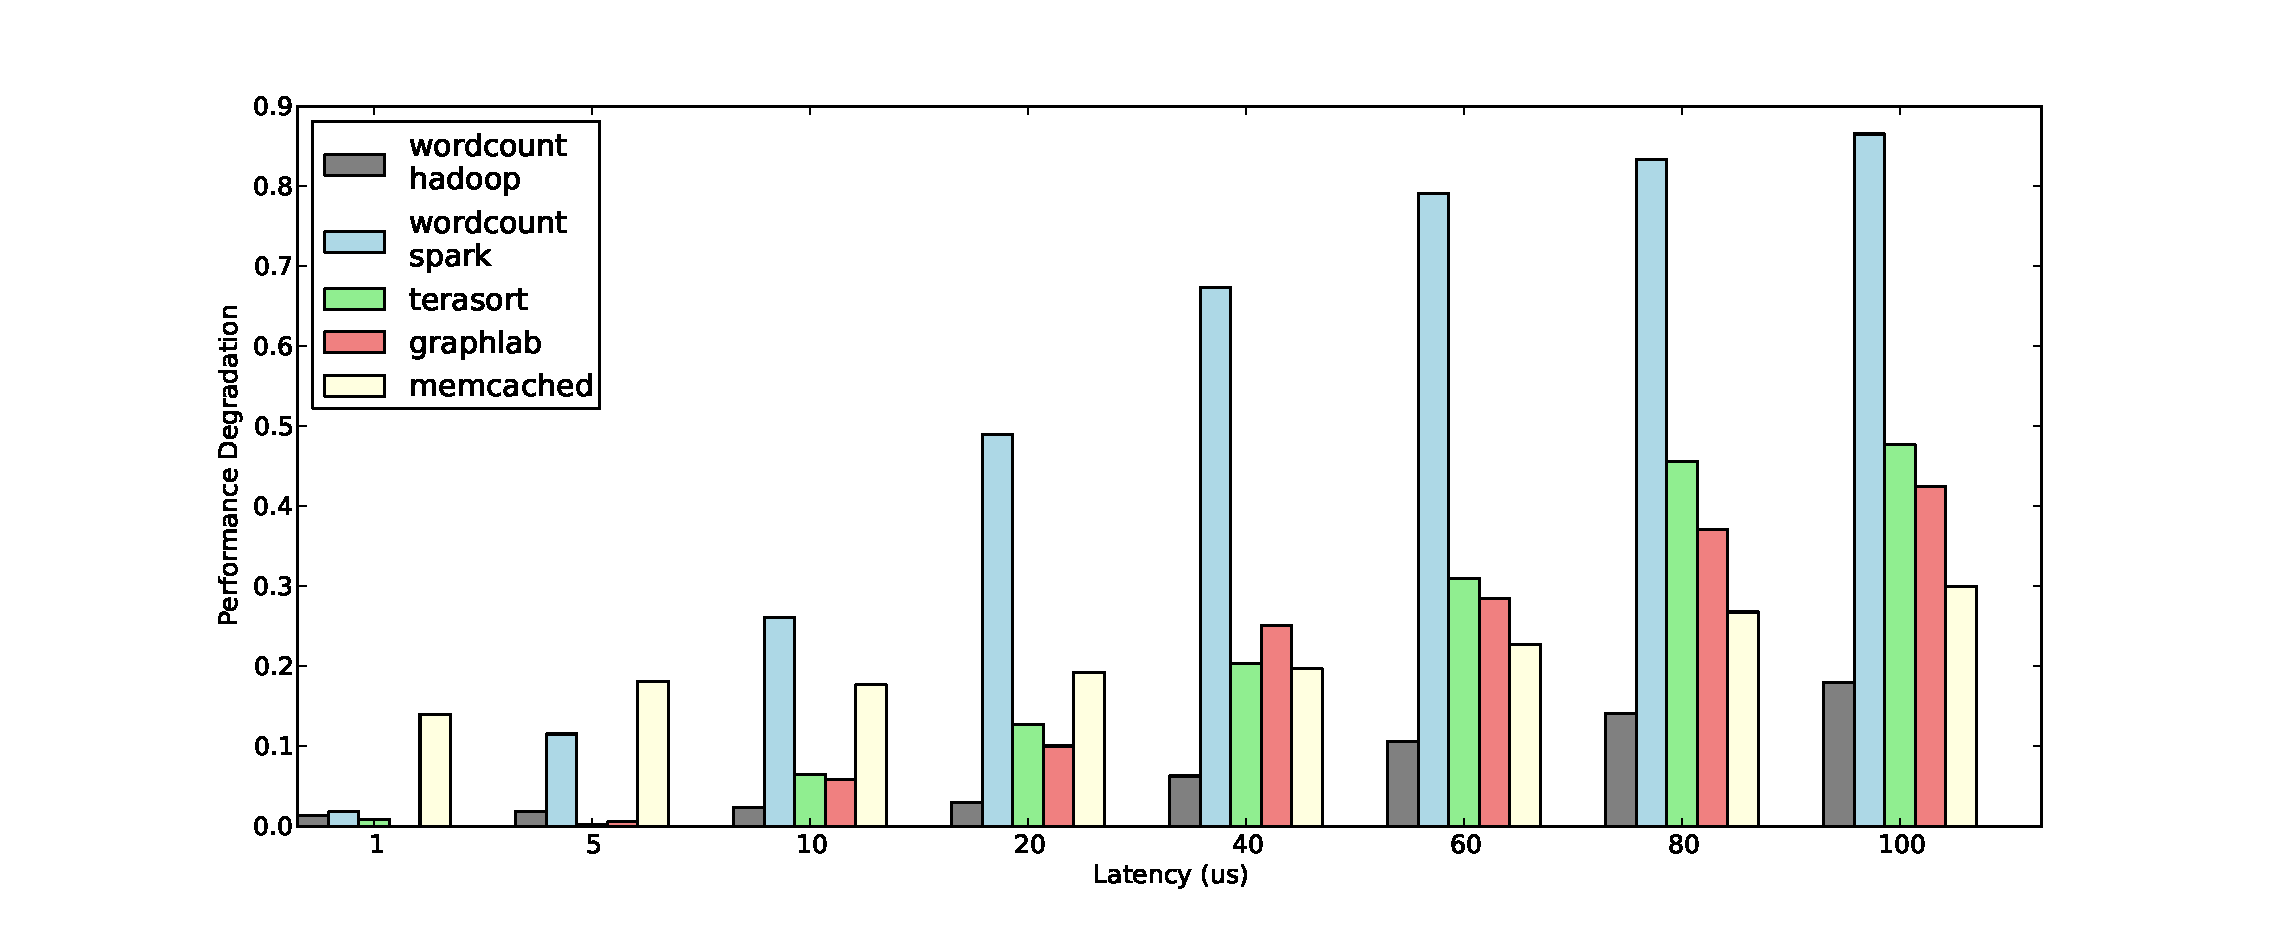
\includegraphics[width = 3.5in]{img/fix_bw_vary_latency.eps} 
  \caption{\small{For a DDC with 40Gbps of bandwidth with varying end-to-end latency, the application performance is sensitive to end-to-end latency.}}
  \label{fig:impl}
\end{figure}
%

One might consider two possibilities to optimizing for latency. First, adopting $100$Gbps technology \emph{not} because we need the higher capacity but instead to reduce transmission and queueing times. E.g., in the event of congestion as in our example above, the packet's transmission time overheads would be reduced from $4\mu$s to $1.6\mu$s. 
The other option is to consider limiting the scope of disaggregation, for example, to within a single rack. Somewhat surprisingly, the potential benefits of this appear modest: the primary impact (to latency) of limiting the scope of disaggregation is to reduce the propagation delay but this already only consumes $1\mu$s from our budget.
(Again, this ignores the potential benefits due to reduced congestion in a rack-scale architecture, which we consider in \S\ref{sec:existing}.)

Finally, a key latency component will arise from software overheads 
at the endpoints. Research prototypes in Xen have reported per-page overheads of $2-6\mu$s, depending on the page replacement algorithm~\cite{ddcHwDesign1} while recent work has argued that such overheads can be reduced to sub-microseconds with the integration of NIC functions into the CPU and software optimizations~\cite{lowlatency}. Thus, while there is reason to believe that software overheads can be optimized to fit within our target latency budget, demonstrating this remains an important topic for future exploration.

\cut{

\paragraphb{Implication \#1:}  The bandwidth requirements for resource disaggregation are within the reach of existing technology. The key enabling factor is a network fabric with low ($\sim 5\mu$s) end-to-end latency.

\vspace{0.1in}
\noindent
%We now discuss the feasibility of a network fabric that provides the above end-to-end latency. Indeed, 
There are two unavoidable contributors to end-to-end network latency --- transmission time for packets in the flow, and propagation delay. \sr{offer evidence??} Given that propagation delays are extremely small in existing datacenters, achieving low end-to-end network latency boils down to minimizing the transmission time for packets in the flow. This has several implications for design of \dis:

\paragraphb{Implication \#2:} Applications running atop \dis must observe little or no queueing delays (that is, no network congestion). 

\vspace{0.1in}
\noindent
The queueing delays observed by flow packets depend heavily on both the network traffic as well as network protocols. We return to evaluating the feasibility of achieving little or no queueing delays in \S\ref{sec:existing}. {motivate via Figure~\ref{fig:impb} and Figure~\ref{fig:impl} $\to$} Note that $100$Gbps links are already available at both switch ports and as server NICs, but are not commonly deployed. Transmission delays dominating the end-to-end network latency have the following implication in the context of \dis:
}

%
\begin{figure}
  \centering
    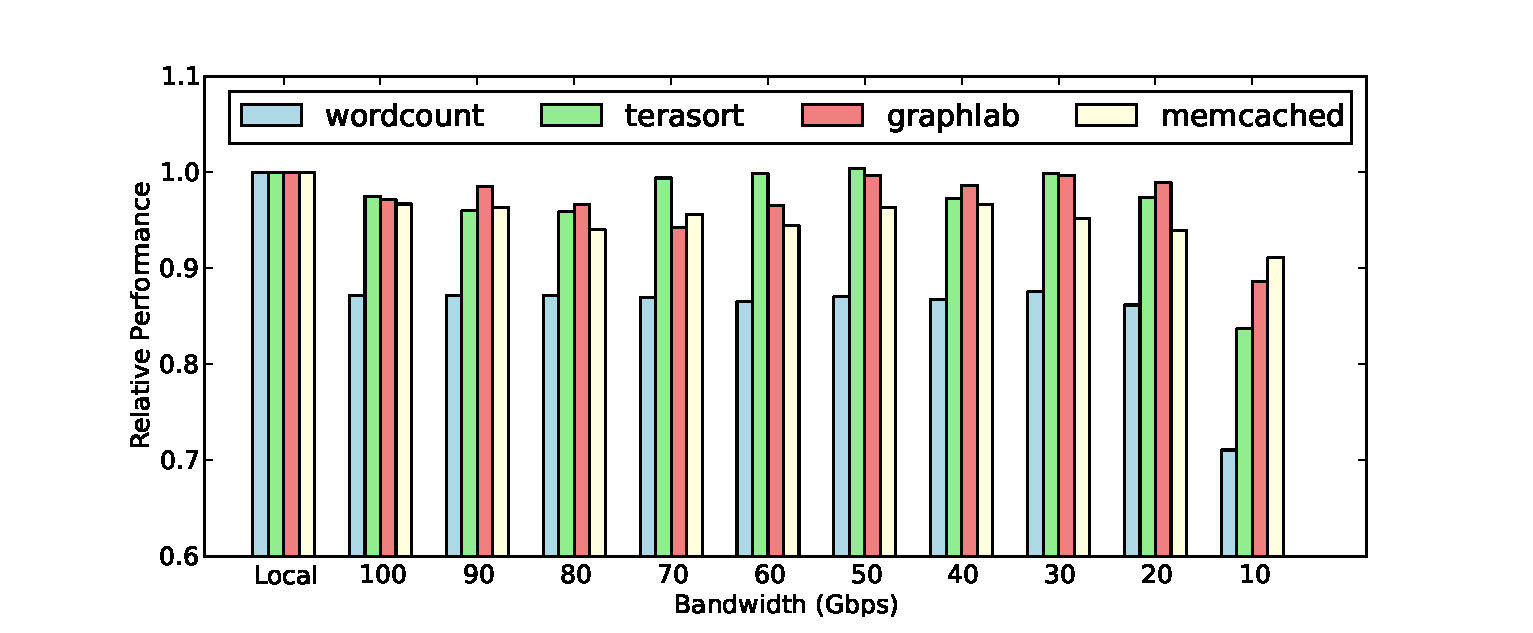
\includegraphics[width = 3.5in]{img/fix_latency_vary_bw.eps} 
  \caption{\small{For a DDC with 5us of end-to-end latency with varying network bandwidth, the network bandwidth has limited impact on application performance after 40Gbps.}}
  \label{fig:impbw}
\end{figure}
%

\cut{
\paragraphb{Implication \#3:} While capacity constraints do not impose strict bandwidth requirements, one good reason to consider $100$Gbps links is reducing end-to-end network latency via reduction in transmission time. 

\vspace{0.1in}
\noindent
 Finally, propagation delays having little impact on end-to-end network latency has an interesting implication in \dis design:

\paragraphb{Implication \#4:} Ignoring congestion, the scale of disaggregation (rack-, pod- or datacenter-scale) may have little impact on application-level performance, and disaggregation at the extreme of datacenter-scale may indeed be feasible.
}

\cut{
\vspace{0.1in}
\noindent
We evaluate the application-level performance for rack- and datacenter-scale resource disaggregation in \S\ref{sec:existing}. 
}

% While $100$Gbps network bandwidth does not provide significant benefits over the $40$Gbps case, reducing the latency down to $1\mu$s can lead to applications observing essentially no performance degradation. In the hindsight, this is not surprising given our results from \S\ref{sec:workloads}, where we established that the network traffic volume does not increase significantly in \dis compared to \pdis, and that the network flows are dominated by short (latency-sensitive) memory access flows. \rc{$\gets$ needs more concrete intuition; remote memory faster than local disk; applications heavily pipelined; CPU bottleneck?}

%\paragraphb{Benefits of remote memory}
%First, given sufficient network bandwidth and small network latencies, use of remote memory can drastically improve application performance compared to traditional disk-based swap. Since the working set size is hard to predict in advance, memory tends to be highly over-provisioned in datacenter servers to prevent thrashing. Disaggregated remote memory can reduce this waste by providing an elastic memory capacity pooled at the datacenter scale. 

% \paragraphb{Reducing latency more important than increasing bandwidth}
% Second, low latency is more important than high bandwidth. The $100$Gbps bandwidth did not provide any significant improvement over the $40$Gbps link. In contrast, $10\mu$s round-trip latency causes noticeable performance degradation, as compared to the $1\mu$s case.


%
% \begin{figure}
%   \centering
%     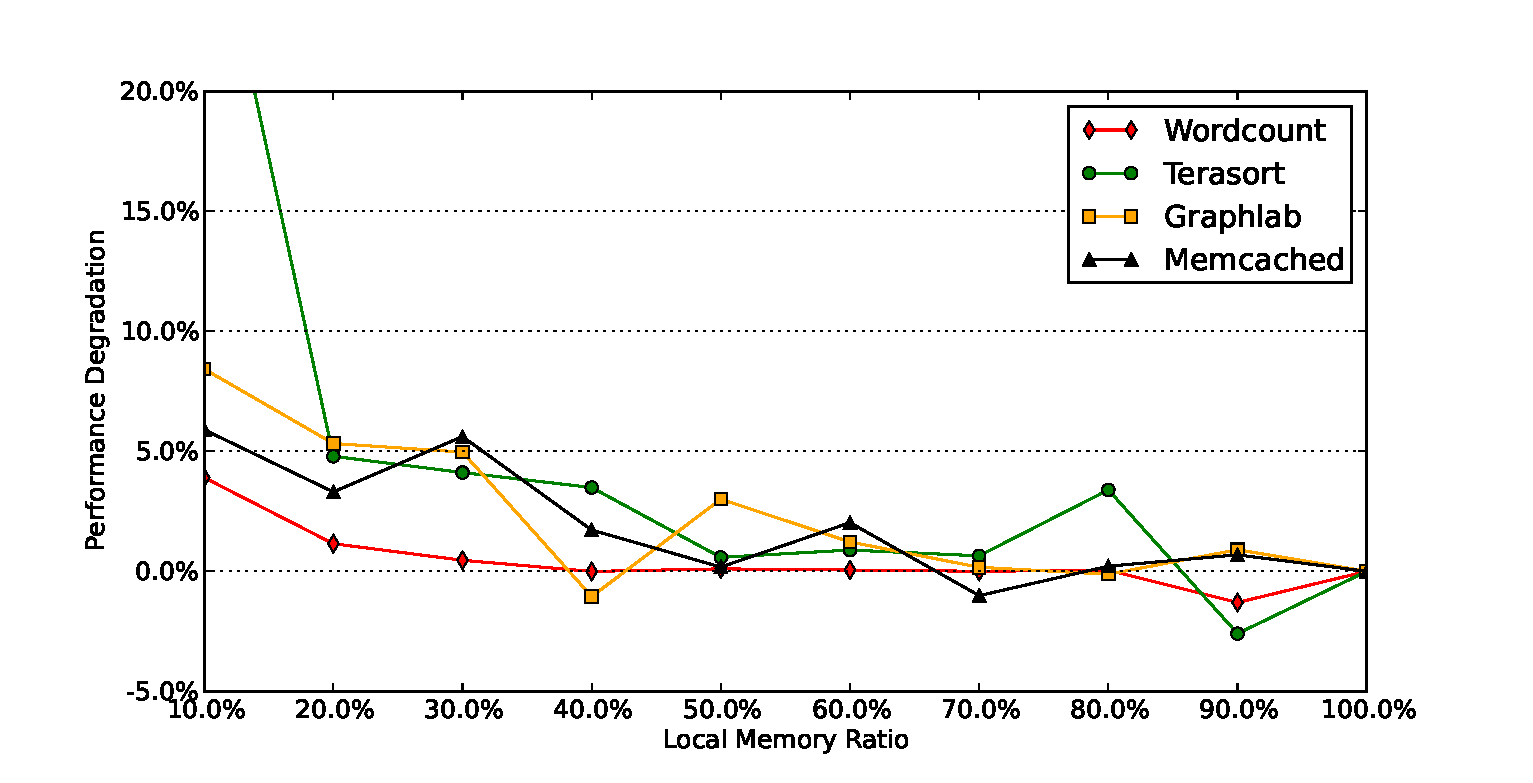
\includegraphics[width = 3.5in]{img/vary_remote_mem.eps} 
%   \caption{\small{\rqc{Fix latency at 5us, bandwidth at 40Gbps, Vary local memory from 0\% to 90\% of the total memory of the EC2 instance}}}
%   \label{fig:impb}
% \end{figure}
%

% graveyard of text scraps.
\cut{
from the network such that the application-level performance in \dis is comparable to that in server-centric architectures.
Overall, our results show that:

\begin{itemize}[leftmargin=*]
	\itemsep0em
	\item CPU blades having local cache is necessary to ensure reasonable performance, given the increased latency to access remote memory. However, $25\%$ of main memory serving as local cache suffices.
	\item Applications require non-trivial latency performance ($5$--$10\mu$s) from the network. In contrast, $40$Gbps access link capacity suffices. Moreover, a good reason to consider higher link capacity is not to handle higher traffic volume, but to reduce the transmission time at the end-hosts.  
    \item Ignoring congestion, the scale of disaggregation (rack versus datacenter scale) has little impact on application-level performance. \rc{$\gets$ right now, we have this results in S5 using simulations for rack and datacenter scale disagg; how should we inject latencies to make this point?}
\end{itemize}

\noindent
}

%Depending on the page eviction algorithm used, 
 %existing research prototypes report this per-page overhead to be roughly in the range of $2$--$6\mu$s~\cite{x1, x2, x3}. However, this overhead can be reduced to sub-microseconds with faster CPUs and software optimization~\cite{y1, y2, y3}, making this overhead insignificant. 
